\section{Methodology}
	The approach undertaken in this study is similar to previous works in the field of applied Machine Learning. Initially, a main theme of the content is selected according to the quality and volume it might produce. In the case of this research, the direction of inquiry is concerned with Tweets relating to the subject of E-Commerce platforms. Such platforms usually see an abundance of Tweets fulfilling the volume requirement. However, additional cleaning steps are taken to insure the informations quality. These cleaning measures are elaborated in the \hyperref[Application]{Application chapter}.
	
	\par
	
	On of the main motives of this research is to observe whether social media data can be evaluated in real-time and distilled into practical knowledge. With this consideration in mind, the data used in this work should bear as much resemblance as possible to a live Tweeter data stream. Acknowledging this consideration, the raw data in the form of Tweets in gathered from the Twitter databases. Namely, the data is collected synchronously, as it is intercepted by the servers. The \textit{Streaming Application Programming Interface} (\cite{stream_api}) is implemented for such use-cases. Employing the \textit{Streaming} API, a connection is established to the servers, which captures a narrow stream (about 15\%) of all Tweets relevant to a given search term. The reduction of stream is due to the complexity in both sending and receiving such a volume of data. Twitter also offers a full non-reduced access through their proprietary \textit{Firehose} API.
	
	\par
	
	The captured data, must then be restructured to fit the data-model of this study, specifically input appropriated for Machine Learning purposes. This includes a preliminary analysis of the data and removal of incomplete observations. The JSON data structure in which Tweets are stored allows for a dynamic non-standard structure, which in turn translates to non-standardized data. Consequently, Tweets must be adapted to conform to a unitary pattern, usually by \textit{flattening} the data into a table. It is also common for Tweets to retrospectively be removed from the Tweeter servers, either by their owners or by Twitter moderators. Such Tweets cannot be analyzed after the fact, since they are no longer available on-line. The process of gathering data and cleansing it is discussed in \hyperref[sec:collect_data]{Part [4.1]}.
	
	\newpage
	
	The next stage entails restructuring the raw captured Tweets into datasets. For this purpose, \textit{features}\footnote{\label{ml_note}Machine Learning nomenclature} are extracted from each observation and converted to a standard array, representing the original Tweet. \textit{Features} are unique properties of the data, which describe it and also possibly its owner, dependent on the approach. Different types of \textit{Features} are used in accordance with the Learning approach undertaken. These approaches are further discussed in \hyperref[build_features]{Part [4.2]}.
	
	\par
	
	The previously constructed features are ensuingly analyzed for consistency and correctness. Subsequently, the features are passed into various Machine Learning algorithms, with the purpose of \textit{training}\footnotemark[1] classifiers. \textit{Training} is the process of deducing the decision rules for classifying the data into one of the categories. This deduction is based on the information the algorithm draws from the input data. Afterwards, the empirical success of these different algorithms will be statistically measured and summarized. Additionally, implications are to be drawn about other use-cases. The classification task observed here is subjective or \textit{fuzzy}\footnote{Fuzzy Logic: A system of logic in which statements do not have to be entirely true or false - \textit{Merriam-Webster Dictionary}} in nature, since the labels themselves are abstract and arguable. Success in this experiment could prove that similarly subjective classification projects are practical. 
	
	\subsection{Training Classifier}
	The purpose of \textit{training} is to create Classifiers. A Classifier is a function, which is fed new observations and automatically recognizes and \textit{labels}\footnotemark[1] them. The intrinsic decision algorithm, through which the Classifier will decide how to allocate a novel observation, usually remains hidden and operates as a black-box of sorts. Seeing that the decision rules could be numerous and considerably not intuitive for human readers, they remain unrevealed. Particularly so, when said algorithms are convolutional. Convolutional Machine Learning schemes, such as \hyperref[ann]{Deep Neural Networks}, may incorporate numerous stages of parameter construction layer-upon-layer, which renders them practically incomprehensible to human users. The actual implementation of all the algorithms would be programmed in the Python programming language and will primarily make use of the scikit-learn module by \cite{scikit-learn}.
	
	\par
	
	The data used for the purpose of this study consolidates 12.520 unique Tweets. Different approaches vary in the percentage of the data used from this corpus. In order to insure robust results, the \textit{Hold-out Method} is used across the board. For each instance of \textit{training} the data is split into two parts - a \textit{training} set and testing set. The \textit{training set} would usually be allocated the larger portion of the data (between 60\% and 90\%) and would be used, as the name suggests for training the classifiers. The remaining corpus chunk (between 10\% and 40\%) would be used for testing the classifiers success. Before each such training-testing session, the data corpus is shuffled. This in turn means, that the training and testing sets constantly differ. This process of splitting, training and testing using different data in each iteration should produce statistically significant results. This method of constantly splitting the data randomly ensures the results robustness.
	
	\par
	
	The following paragraphs expand on the different Machine Learning schemes. Figure \ref{fig:classifier_matrix} illustrates these schemes with relation to computational complexity and their interoperability.
	
	\begin{figure}[h]
		\centering
		%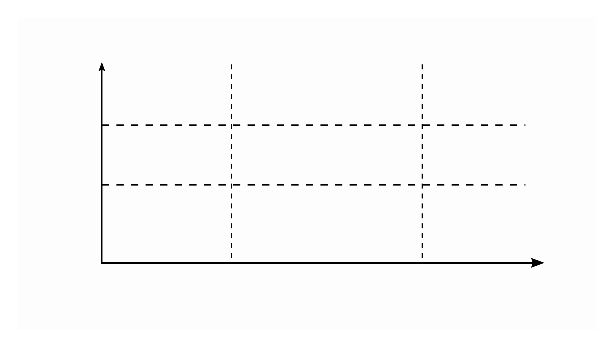
\includegraphics[width=0.8\textwidth]{methods}
		\scalebox{1.0}{\input{images/methods.eps_tex}}
		\captionsetup{width=0.8\textwidth}
		\caption{Clustering of Different Classifiers}
		\label{fig:classifier_matrix}
	\end{figure}
	
	\subsection{Supervised Learning}
	\label{classifer_types}
	
		\subsubsection{Regressions}
	Probably the most basic approach is simply running a regression with all the features as the independent variables and the a numeric representation of the classes as the dependent variable. Such an approach is shown in Equation \ref{regression}. Some threshold value between the classes must be determined since the estimate for the explained variable, will have a non-deterministic value. Regressions are primarily to be used as a benchmark for the other algorithms to measure up against.
	
	\begin{equation}
		\mathbb{E}(\hat{y} \ \vert \ \textbf{x}) \approx 
		\begin{cases}
			label = \text{News}, &\hat{y} \geq y^* \\
			label = \text{Not News},\ \ &\hat{y} < y^*
		\end{cases}
		\label{regression}
	\end{equation}
	
	\par
	\paragraph{Linear Regression}
		This method builds a linear dependency system between the explained variable (in this case, a numerical representation of the Class) and the explaining variables (Features). With the \textit{Bag-of-Words} approach, each parameter \textit{x} is a dummy variable indicating whether a given word \textit{m} is present in Tweet \textit{i}. The estimations parameters, which are denoted with $\beta_j$ are derived using Ordinary Least Squares. In itself, the linear regression estimation is a weak predictor for the purpose of classification, but it allows for calculating other useful statistics such as the coefficient of determination, commonly known as $R^2$. This static demonstrates the part of the variance that is explained using the provided variables and is also called 'goodness of fit'. We therefore strive to maximize it as much as possible. The more variance covered by our variables, the better we are able to predict the outcome of the classification. 
		
		\begin{figure}[h]
			\centering
			%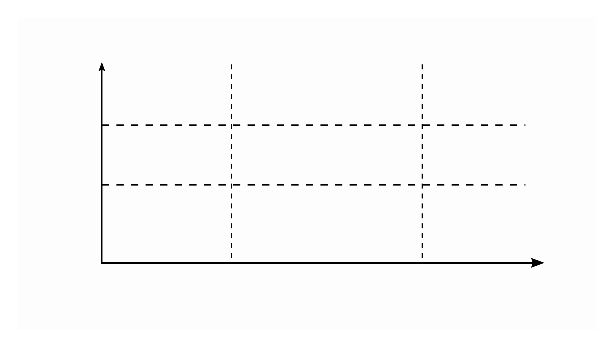
\includegraphics[width=0.8\textwidth]{methods}
			\scalebox{0.8}{\input{images/red_dist.eps_tex}}
			\captionsetup{width=0.8\textwidth}
			\caption{Distribution of predicted $ \hat{y} $ around the labels}
			\label{fig:y_dist_reg}
		\end{figure}
		
		Another point of interest is the distribution of predicted classifications $\hat{y}$. In an ideal scenario, the distribution of $\hat{y}$ would be concentrated around the numerical representations of the classes as in Figure \ref{fig:y_dist_reg}. The basic premise for the use of linear regressions as classification tools, where $ n $ is the number of observations, $ m $ is the number of features as presented in Equation \ref{lin_reg}.
	
	\begin{equation}
		y_i = \beta_1 x_{1i}+ \beta_2 x_{2i} + ... + \beta_m x_{mi} + \epsilon_i \ \ \ \ \ \ \ \ 
		\forall \ i \in [1,n].
		\label{lin_reg}
	\end{equation}
	
	\paragraph{Logistic Regression} Despite its name, the actual regression model executed here is linear, and is used primarily for classification rather than regression analysis (\cite{bishop2006logistic}). This regression scheme differs from linear firstly, in the fact, that the possible outcomes of the dependent variable are discreet rather than continuous. Secondly, the probabilities which describe the different outcomes of a regression instance, are modeled using a logistic function. The discrete outcomes can in turn be converted to labels, which in allows for a more fluent application as a classification tool and is therefore commonly employed in  Machine Learning. Logistic regression analysis is formally represented as follows in Equation \ref{logit}. The $x$ vector represents all explanatory variables, in our case, the Tweet features. The term error $\epsilon$ follows the standard logistic distribution, which also gives the regression its name. 
	
	\begin{equation}
		y = 
		\begin{cases}
		1 \ \  \beta_0 + \beta_1 x + \epsilon > 0 \\
		0 \ \  \text{else } 
		\end{cases} \text{         } \forall \  x = 
		\begin{pmatrix}x_1\\x_2\\...\\x_n \end{pmatrix}
		\label{logit}
	\end{equation}
	\subsubsection{Naive Bayes}
	Probably the most common classification algorithm and usually the go-to classifier when handling text classification tasks [\cite{rish2001empirical}]. The Naive Bayes algorithm is popular because its tends to perform as good as much more complex classifiers, if not outperform them. This being true despite the overly simplified or "naive" assumptions being made at the core of the classifier. This algorithm is prevailing for different text classification problems such as: sentiment analysis, spam filtration and classifying text segments to user-defined classes as in my case. Te approach taken with this classifier is probabilistic, since it classifies an observation according to which class is it most likely to belong to given its features. 
	The word "Naive" in its name come from its base assumption, which is that the occurrence of a certain feature in a data point is independent from the the occurrences of other features. Therefore the probabilistic calculus is as in [\ref{nb_calc}], where $ \textbf{X} = (x_1,...,x_n) $ is a vector of the data points features and $ C $ is the appropriate class.
	
	\begin{equation}
		P(\textbf{X}|C) = \prod_{i=1}^n P(x_i|C)
		\label{nb_calc}
	\end{equation}
	
	\paragraph{Classification}
		At its heart, the algorithm is based on Bayes theorem [\ref{nb_bayes}], which allows for the calculation of conditional probability. In the case of classification, it is the probability that a novel data point belong to a given class $ C_i $ given its describing properties (features) $ \textbf{X} $.
	
	\begin{equation}
		P(A|B) = \frac{P(X|A) \cdot P(A)}{P(B)}
		\label{nb_bayes}
	\end{equation}
	
		The algorithm thus calculates the posterior probability of the data point to be part of each given class $ i $  out of $ k $ classes. After which these probabilities are than compared [\ref{nb_post_prob}]. The classification of the new point is determined by which class is most likely (has the highest probability). In order to calculate these likelihoods, we first calculate the numerator of [\ref{nb_post_prob}] as in [\ref{nb_prob_numerator}]
	
	\begin{equation}
		\begin{aligned}
			P(C_i|x_1, ... , x_n) &= \frac{P(x_1, ... , x_n |C) \cdot P(C_i)}{P(x_1, ... ,x_n)} \\
			& \ \forall \ \ \  1 \leq \ i \leq \ k
		\end{aligned}
		\label{nb_post_prob}
	\end{equation}
	
		In [\ref{nb_prob_numerator}] we derive that the conditional probability term, $ P(x_j|x_{j+1}, ...,x_n,C_i) $ is equal to $ P(x_j|C_i) $ based on the assumption that the occurrence of certain features $ j $ is independent of the occurrences of all other features $ (x_1,x_2,..., x_{j-1},x_{j+1}, ...,x_n) $ [\ref{nb_calc}].
	
	\begin{equation}
		\begingroup\makeatletter\def\f@size{8}\check@mathfonts
			\begin{aligned}
				P(x_1,x_2, ..., x_n |C) \cdot P(C_i) &= P(x_1,x_2,...,x_n,C_i) \\
				P(x_1,x_2, ..., x_n,C_i) &= P(x_1|x_2, ...,x_n,C_i) \cdot P(x_2, ...,x_n,C_i) \\
				&= P(x_1|x_2, ...,x_n,X_i) \cdot P(x_2|x_3, ..., x_n, C_i) \cdot P(x_3, ..., x_n,C_i) \\
				&= \ ... \\
				&= P(x_1|x_2, ...,C_i) \cdot P(x_2|x_3, ...,C_i) \cdot ... \\
				& \ \ \ \ \ \ \ \ \ \ \ \ \ \ \ \ \ \ \ \ \ 
				... \cdot P(x_{n-1}|x_n, ...,C_i) \cdot P(x_n|C_i) \cdot P(C_i)
			\end{aligned}
		\endgroup
		\label{nb_prob_numerator}
	\end{equation}
	
		The calculation in equation[\ref{nb_prob_numerator}] allows us to formulate the classification equation results in equation [\ref{nb_final}].
	
	\begin{equation}
		\begin{aligned}
			P(C_i|x_1,x_2, ...,x_n) &= \Bigg(
			\prod_{j=1}^n  P(X_j|C_i)
			\Bigg) \cdot
			\frac{P(C_i)}{P(x_1,x_2, ..., x_n)}\\ 
			&\ \forall \ \  1 \leq i \leq k \\
			\text{The expression } P(&x_1,x_2, ...,x_n)\text{ is constant for all classes } j: \\
			P(C_i|x_1,x_2, ...,x_n)& \propto \Bigg(
			\prod_{j=1}^n  P(X_j|C_i)
			\Bigg) \cdot P(C_i) \\
			&\ \forall \ \  1 \leq i \leq k 
		\end{aligned}
		\label{nb_final}
	\end{equation}
	
	\paragraph{Variations of the Algorithm}
		Several algorithms, which are derivative forms of the basic Naive Bayes algorithm are also quite common. These variations usually implement different distributions on the feature probability $ P(x_j|C_i) $.
		
		\subparagraph{Gaussian}
			A natural assumption when handling continuous data is that the values associated with each class are also continuous and distributed normally. De facto, the data is first segmented by the class $ c_i $. Following, the mean and variance of each continuous variable $ x_j $ for each class  $ c_i $. Let $ \mu_i $ and $ \sigma_i^2 $ be the mean and variance of feature set $ x $ associated with class $ C_i $ accordingly. The algorithm assumes a normal (Gaussian) distribution for the features, where as the parameters $ \sigma_i $ and $ \mu_i $ are derived from a maximum likelihood estimation, i.e.,
	
		\begin{equation}
			P(x_j|C_i) = \frac{1}{\sqrt{\vphantom{\frac{1}{1}} 2 \pi \sigma^2 c_i}} \cdot 
			\scaleobj{2}{e}^{ \displaystyle - \frac{(x_j-\mu c_i)^2}{2 \sigma^2 c_i} }
		\end{equation}
	
		\subparagraph{Multinomial}
			Here the features represent the frequencies of word occurrences which are distributed in a multinomial fashion such that $ p_i $ is the probability that an event $ i $ occurs in the multinomial $ (p_1,p_2, ...,p_n) $. The feature set $ \textbf{x} = (x_1,x_2m ...,x_n) $ can than be visualized as a histogram, in which the frequency of event $ i $ (appearance of word $ i $ in a given data point) is represented by the hight of the appropriate column. This method is especially common when undertaking the Bag of Words approach. This will be further demonstrated in the Application part. Therefore, the likelihood of generating a histogram \textbf{x} is represented in [\ref{nb_multinom}].
	
	\begin{equation}
		P(X|C_k) = \frac{(\sum_i)!}{\prod_i x_i !} \cdot \prod_i p_{ki}^{x_i}
		\label{nb_multinom}
	\end{equation}
	
		When extrapolated into log-space, [\ref{nb_multinom}] turns into [\ref{nb_multinom_log}], where $ b = log \big( P(C_k)\big) $ and $ \textbf{w}_{ki} = log \big( p_{ki} \big) $. It is now evident that the classifier becomes linear in logarithmic-space.
	
	\begin{equation}
		\begin{aligned}
			log \big[ P(X|C_k) \big] &\propto log \bigg( P(C_k)\prod_{i=1}^n p_{ki}^{x_i} \bigg) \\
			&= log \bigg(P(C_k) \bigg) + \sum_{i=1}^n x_i \cdot log(p_{ki}) \\
			&= b + \textbf{w}_k \cdot \textbf{x} 
		\end{aligned}
		\label{nb_multinom_log}
	\end{equation}
		
		Additionally, the product must be adjusted for the case when a certain event (appearance of word $ i $) does not occur. Since non-occurrence will be denoted as a frequency equal to zero, such values must be smoothed out to prevent them from nullifying the entire equation.
	
	\subparagraph{Bernoulli}
		This variant assumes multivariate Bernoulli distributions for the features. Particularly, each feature can be represented with a boolean variable. Hence, the classifier requires the feature sets to passed in the form of vectors composed of binary variables each representing a feature. The classification is based on the decision rule in [\ref{nb_bernoulli}], for class $ C_k $ and feature $ x_i $. The probability of class $ C_k $ producing the feature $ x_i $ is denoted by $ p_{ki} $. We can see that the non-occurrence problem from the Multinomial variant is being explicitly addressed here by penalizing for non-occurrence of a given feature $ x_i $.
	
	\begin{equation}
		P \big(\textbf{x}|C_k \big) = \prod p_{ki}^{x_i}(1-p_{ki})^{(1-x_i)}
		\label{nb_bernoulli}
	\end{equation}
	\subsubsection{Support Vector Machines}
	\label{svm}
	
	\paragraph{Background}
	The original Support Vector Machine (SVM) algorithm was formulated by Vladimir N. Vapnik and Alexey Ya. Chervonenkis in 1963 while working at the institute of Control Sciences in Moscow. Despite the theory behind SVM's being far from new today, it remained mostly theoretical until quite recently. The state of technology at the time of its conception was far behind the theory, and it would take decades until computers would reach the computational abilities that could facilitate SVMs.
	
	\paragraph{Implementation}
	SVM aims at segmenting an input dataset to binary categories (\cite{SVM_burges1998tutorial}). For example, positive and negative observations or analogously membership in or absence from a certain category. A common example is whether a given Email should be classified as Spam or not by the mail server. The rational behind SVMs could best be visualized by imposing the training observation on two dimensional Euclidean space (Figure \ref{svm_euclidean_space}) and then generalized to $ n $ dimensions.
	
	\begin{figure}[h]
		\centering
		%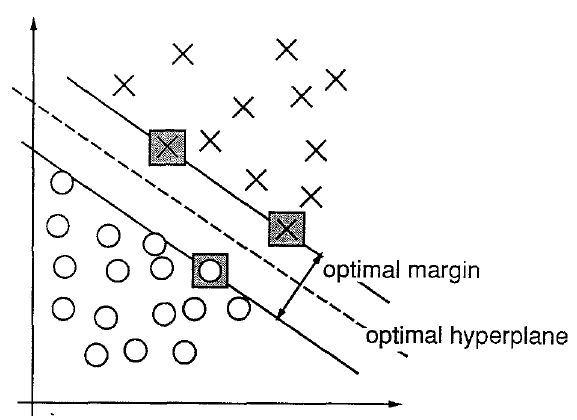
\includegraphics[width=0.8\textwidth]{svm.png}
		\scalebox{0.8}{
			\input{images/svm_euclidean_space.eps_tex}
		}
		\captionsetup{width=0.8\textwidth}
		\caption[SVM in Euclidean Space]{
			\footnotesize{
				Euclidean Imposition of data. The support vectors, marked with grey squares, define the margin of largest separation between the two classes. \textit{Source:} \cite{SVM_cortes1995support}.
			}
		} 
		\label{svm_euclidean_space}
	\end{figure}

	 The algorithm strives to define a dividing line, which would create a separating threshold between the two groups. In two-dimensional space, the separator is demarcated using a simple line (dashed line in Figure \ref{svm_euclidean_space}). Said line is then positioned in a manner, creating maximal (optimal) separation between the two groups. This is achieved by drawing parallels through the closest positioned members of both groups. The linear divider lays in the middle between this two parallels. The observations which are positioned on the parallels themselves, define the \textit{curbs} of the so-called \textit{dividing street}, and are dubbed Support Vectors (gray squares in the Figure). From them in turn, the algorithm derives its name. Any new observation passed to the trained classifier for assignment, will be allocated to the appropriate group, as is defined by its position relative to the separating hyperplane. 
	
	 A dataset of size $n$, as in Equation \ref{svm_div_line}, is to be used as a training set, in which $y_i$ stands for the actual class of the observation $i$ and can have one of either values $y_i \in [+1;-1] $. The values represent a positive and negative classification accordingly. A positive $(+1)$ classification implies the presence of the sought-after class, $News$ in our case. The vector $(\textbf{x}_i)$ is an array of size $p$, representing the features which compose each observation. In the 2-dimensional example, the 2 features of $(\textbf{x}_i)$ can be graphically illustrated in euclidean space as the $(x,y)$ coordinates $(\textbf{x}_i) = [x_i^{(1)},x_i^{(2)}]$. 
	 
	\begin{equation}
		\begin{aligned}
			(\textbf{x}_1,y_1),& ... , (\vec{x}_n,y_n), \ \ y \in \big[-1;+1 \big] \\
			\textbf{x}& = (x_{i1},x_{i2}, ...,x_{ip})
		\end{aligned}
	\label{svm_div_line}
	\end{equation}
	
	The optimal hyperplane segregates the two data classes, creating a maximally wide barrier between the closest observations of the opposing classes. This hyperplane is delineated in Equation \ref{svm_optimum}. The vector $\vec{w}$ is the normal vector\footnote{A vector perpendicular to a given object, the diving hyperplane in this case} to the dividing hyperplane and the parameter $b$ represents the normal vector's offset along the axis. The area enclosed between the 2 hyperplanes, defined by the support vectors, is referred to as the \textit{optimal margin}. These support vectors are illustrated in Equation \ref{svm_supp_vecs}.
	
	\begin{equation}
		\begin{aligned}
			\vec{w}& \cdot \textbf{x} - b = 0 \\
			\vec{w}& = (w_1, ... , w_p) 
		\end{aligned}
		\label{svm_optimum}
	\end{equation}
	
	\begin{equation}
		\vec{w} \cdot \textbf{x} - b = 
		\begin{cases}
			+1 \\
			-1 
		\end{cases}
		\label{svm_supp_vecs}
	\end{equation}
	
	The distance between any point and the separating line (Equation \ref{svm_optimum}) is shown in Equation [\ref{svm_dist}]. The distance between the 2 hyperplanes is equal to twice the distance between the support vectors and the separating line, hence $ \frac{2}{||\vec{w}||} $. The optimization problem at hand is thus the maximization of this distance, in order to create a maximally distinct margin between the classes. Furthermore, no observation from the training data can be positioned inside the margin designated in Equation \ref{svm_constaints}.
	
	\begin{equation}
		\begin{aligned}
			\text{Dist.}&\text{ for some point i}: \\ 
			&\frac{| \textbf{x}_i \cdot \vec{w} + b|}{||\vec{w}||},
		\end{aligned}
		\ \ \ \Rightarrow 	\ \ \ \ 
		\begin{aligned}
			\text{Dist.}&\text{ for support vectors:} \\
			&\frac{w^T\textbf{x} + b}{||\vec{w}||} = \frac{\pm 1}{||\vec{w}||}
		\end{aligned}
		\label{svm_dist}
	\end{equation}
	
	\begin{equation}
		\text{or}
		\begin{aligned}
			\vec{w}& \cdot \textbf{x} - b \geq 1 \ \ \forall \ \  y_i = +1 \\
			\vec{w}& \cdot \textbf{x} - b \leq 1 \ \ \forall \ \  y_i = -1
			\end{aligned}	
			\ \Rightarrow \ 
			\begin{aligned}
			y_i(&\vec{w} \cdot \textbf{x}_i - b) \geq 1 \\
			&\forall \ 1 \leq i \leq n
		\end{aligned}
		\label{svm_constaints}
	\end{equation}
	
	Finally, the core optimization problem is to enlarge the margin as much as possible, subject to all the training data points being located on the correct side of the margin, given their actual class. As denoted in Equation \ref{svm_opt_dist}.
	
	\begin{equation}
		\begin{aligned}
			&max \Bigg(\frac{2}{||w||}\Bigg) \Rightarrow 
			min \Bigg( \frac{w^Tw}{2}	\Bigg)\\
			&subject \  to \ \ y_i(\textbf{x}_i \cdot w + b) \geq 1
		\end{aligned}
		\label{svm_opt_dist}
	\end{equation}
	
	The optimal solution is array of values $\alpha$, which are the learned weights to the $x$'s and are equal zero for all but the support vectors ($y_i = \pm1 $). Incorporating the line Equation \ref{svm_div_line} results in Equation \ref{svm_opt_dist2}.
	
	\begin{equation}
		w = \sum_{i=1}\alpha_i y_i \textbf{x}_i \ \ \ \xRightarrow[]{(\ref{svm_div_line})}
		\ \ \ w \cdot \textbf{x} + b = \textbf{x} \cdot  \sum_{i=1} \alpha_i y_i \textbf{x}_i  + b
		\label{svm_opt_dist2}
	\end{equation}
	
	It is now possible to derive a classification function based on the previous results. When classifying new data, unseen novel observations might fall inside the $[-1:+1]$ margin, and are therefore classified according their sign (positive/negative) as in Equation \ref{svm_sgn_function}.
	
	\begin{equation}
		f(x) = \text{sgn}(\vec{w} \cdot \textbf{x} + b)  =
		\text{sgn}\bigg( \sum_{i=1} \alpha_i
		\xunderbrace{
		 \xoverbrace{\textbf{x}_i}^{\substack{\text{New}\\ \text{Obs.}}}
	  \cdot 
	  \xoverbrace{\textbf{x}}^{\substack{\text{Support}\\ \text{Vectors}}}
		}_{dot \ product}
		 + b \bigg)
		\label{svm_sgn_function} 
	\end{equation}
	
	Notice that the results of the classification function depends solely on the dot product between the vector of the new point and the support vectors $(\textbf{x} \cdot\textbf{x}_i)$. It is hence possible to classify as shown in Equation \ref{svm_classification}.
	
	\begin{equation}
		\text{class}(x) = 
		\begin{cases}
			positive,\ \ \  &f(x) > 0 \\
			negative,\ \ \  &f(x) < 0
		\end{cases}
		\label{svm_classification}
	\end{equation}
	
	The basic SVM classification algorithm in itself seems to present a solution to a very limited spectrum of classification problems, that is two-dimensional, linearly-separable binary class classification problem. The following paragraphs present solutions to each on of these difficulties, through generalization of the basic algorithm. Notice that replacing the dot product from Equation \ref{svm_sgn_function} can be generalized to any number $\mathbb{Z}^+$ of dimensions, clearing the dimensionality restriction. The \textbf{Kernel Trick} resolves the linear-separability problem, by mapping to a higher dimension.
		
	\par		
	\paragraph{Kernel Trick}
	A key element of SVMs statistical and computational power is the Kernel Trick (\cite{guyon1993automatic}). Using the Kernel-Trick, the linearly dimensional training data $x$ are extrapolated onto a higher plane using a mapping function $\Phi:\textbf{x} \rightarrow \varphi(x)$, with the assumption that on the new plane a better linear separating hyper plane can be found. The mapping is carried out using a \textit{kernel trick}, where by the internal dot product of the linear separator is replaced with a Kernel Function. This function simulates the redistribution of the original Support Vectors in a richer space, barely incurring an additional computational cost in the process. The linear separator in the new space is not bilinear on the original plane, thus the classification of new observation is also done using the Kernel Function. Whence the data is still not separable using a hyperplane in the new space, the dataset can be mapped to a higher still dimensional space. Mapping to a higher dimension is illustrated in Equation \ref{svm_phi_x}.
	
	\begin{figure}[h]
		\centering
		\captionsetup{width=0.8\textwidth}
		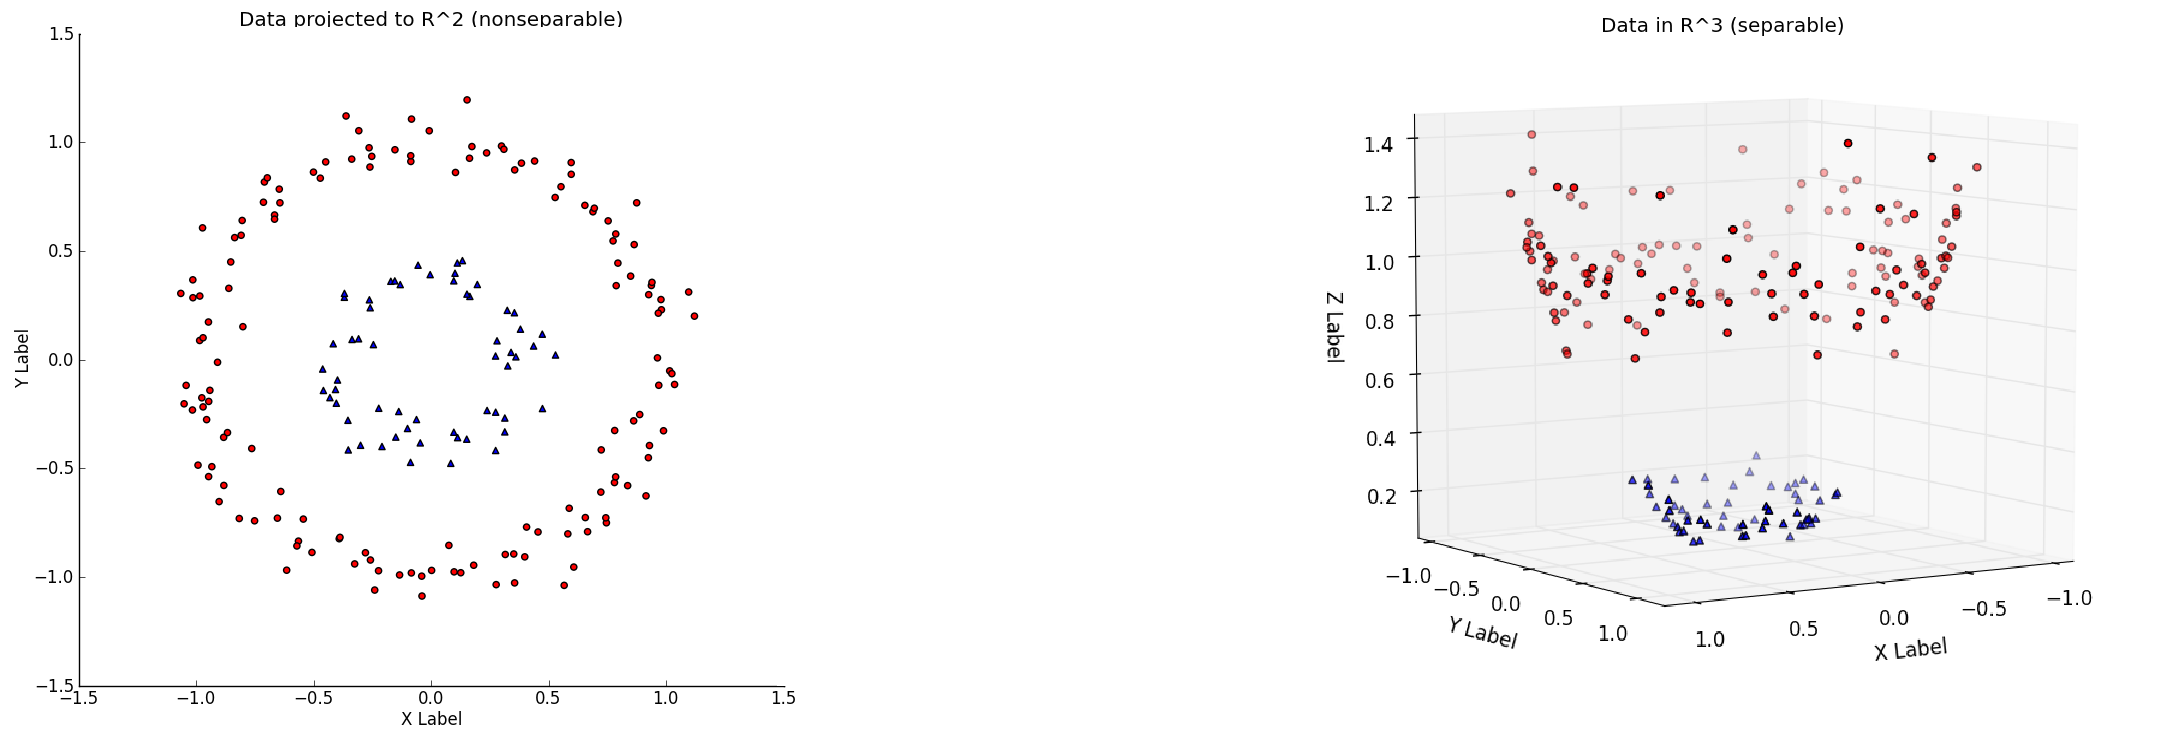
\includegraphics[width=0.8\textwidth]{data_2d_to_3d}
		\caption[SVM Dimensionianl Extrapolation]{
			\footnotesize{
				(Left) A dataset in  , not linearly separable. (Right) The same dataset transformed:
				$\varphi \big(x_1, x_2\big) \Rightarrow \big[ x_1,x_2,x_1^2+x_2^2 \big]$.
				\textit{Source}: \cite{kimso}
			}
		}
	\end{figure}

	\begin{equation}
		\begin{aligned}
			\mathlarger{\Phi}: \textbf{x} \ \ &\rightarrow \ \  \varphi(\textbf{x}) \\
			\mathlarger{K}(\textbf{x}) &\rightarrow \ \varphi(\textbf{x}_j)^T \varphi(\textbf{x}_j)
		\end{aligned}
		\label{svm_phi_x}
	\end{equation}
	
	\begin{equation}
		\sum_{i=1} \alpha_i y_i (\textbf{x}_i^T \textbf{x}) + b  \ \  \rightarrow \ \ 
		\sum_{i=1} \alpha_i y_i \mathlarger{K}(\textbf{x}_i, \textbf{x}) + b
		\label{svm_insert_kernel}
	\end{equation}
	
	The function K in Equation \ref{svm_insert_kernel} represents a kernel function and acts as a similarity measure which corresponds to the inner product in some higher feature space. As long as there exists a dimensional space of greater magnitude, in which the kernel function is the dot product of that higher dimensional space, such a kernel is in fact a dot product, and as such can be classified using the normal linear classifier without loss of generality. Several possible kernel functions are demonstrated next.
	
	\par	
	
	\paragraph{Linear Kernel}
		The kernel is in simply the dot product (Equation \ref{svm_lin_kernel}) and must not be mapped to a higher dimension. Therefore, the number of dimensions stays the same $ \mathbb{N} \rightarrow \mathbb{N} $.
		\begin{equation}
			\mathlarger{K}(x_i,x_j) = x_i^T x_j
			\label{svm_lin_kernel}
		\end{equation}
	
	\paragraph{Polynomial Kernel}
		Training data is extrapolated using a polynomial kernel function (Equation \ref{svm_poly_kernel_def})] into a higher dimensional space. The kernels represents the similarity of training samples in a feature space over polynomials of the original variables, allowing learning of non-linear models. Additionally, the polynomial kernel adds an interpretive intuition by applying interaction variables (products of $ x_i $ and $ x_j $).
		
		\begin{equation}
			\begin{aligned}
				\mathlarger{K}(\textbf{x}_i,\textbf{x}_j) = {(r + \gamma \cdot \textbf{x}_i^T \textbf{x}_j)}^d, \ \ \forall \gamma > 0 
			\end{aligned}
		\label{svm_poly_kernel_def}
		\end{equation}
		
		In Equations \ref{svm_poly_kernel_R2}, \ref{svm_poly_kernal_proof} it is demonstrated that substituting the dot product with a kernel function results in the dot product on a higher dimension. Specifically Equation \ref{svm_poly_kernal_proof} demonstrates the extrapolation of $ d=2 $ space to $ d=6 $ by employing a polynomial function.
		
		\begin{equation}
			\begin{aligned}
				&\text{Let   } \mathlarger{K}(\textbf{x}_i,\textbf{x}_j) = {(1 + \textbf{x}_i^T \textbf{x}_j)}^2 
				&\text{such that   } \textbf{x}: \mathbb{R}^2 \Rightarrow \mathbb{R}^6
			\end{aligned}
			\label{svm_poly_kernel_R2}
		\end{equation}
		
		\begin{equation}
			\begin{split}
				\mathlarger{K} \xoverbrace{(\textbf{x}_i,\textbf{x}_j)}^{\mathbb{R}^2}
				&= {(1 + \textbf{x}_i^T \textbf{x}_j)}^2 \\
				& = 1+ x_{i1}^2 x_{j1}^2 
				+ 2 \big(x_{i1}x_{j1} +  x_{i1}x_{j1}x_{i2}x_{j2} + x_{i2}x_{j2}\big) 
				+ x_{i2}^2 x_{j2}^2 \\ 
				& = \big[
					1 + x_{i1}^2 + \sqrt{2}x_{i1}x_{i2} + x_{i2}^2 + \sqrt{2}x_{i1} + \sqrt{2}x_{i2}
				\big]^T
				\cdot \\
				&\hspace{2cm} \big[
					\underbrace{1 + x_{j1}^2 + \sqrt{2}x_{j1}x_{j2} + x_{j2}^2 + \sqrt{2}x_{j1} + \sqrt{2}x_{j2}}_{\mathbb{R}^6}
				\big] \\
				&= \varphi(x_i)^T\varphi(x_j) \\ 
				\text{such that :}&\\
				 \varphi(x) &= \big[
					 \xoverbrace{1 + x_1^2  + \sqrt{2}(x_1 + x_1x_2 + x_2) + x_2^2}^{\mathbb{R}^6}
				 \big]
			\end{split}
			\raisetag{2\normalbaselineskip}
			\label{svm_poly_kernal_proof}
		\end{equation}
		
	\paragraph{Gaussian Radial Basis Kernel}
		The Radial Basis Function (RBF) is a prevalent kernel in Machine Learning algorithms.
		\begin{equation}
			 \begin{aligned}
				\mathlarger{K}(\textbf{x}_i,\textbf{x}_j) = \mathlarger{\mathlarger{e}}^{
					\displaystyle  -\Bigg(
					\frac{||\textbf{x}_i - \textbf{x}_j||^2}{2 \sigma^2}
					\Bigg)}& \ \ \
				\overset{\mathclap{\tikz \node {$\downarrow$} node [above=1ex] {$\gamma = \frac{1}{2\sigma^2}$};}}{=}
				\mathlarger{\mathlarger{e}}^{\displaystyle  -\big(
					\gamma \cdot ||\textbf{x}_i - \textbf{x}_j||^2
					\big)}, \\
				& \forall \gamma \ > 0 
			 \end{aligned}
		\end{equation}
		The value of the RBF kernel function ranges from zero (in the limit) to one (when $\textbf{x}_i = \textbf{x}_j$) and declines as the distance between the points grows smaller. RBF is likewise interpreted as a similarity measure, which is why it fits well to the kernel function idea. The feature space of the kernel is of infinite dimensionality.
		
	\paragraph{Sigmoid Kernel}
		The Sigmoid function, also known as the Hyperbolic Tangent function, bares semblance to the behavior of the logistic regression by creating an "S"-shaped curve (Figure \ref{fig:svm_sig_kernale}). 
		
		\begin{figure}[h]
			\centering
			\captionsetup{width=0.8\textwidth}
			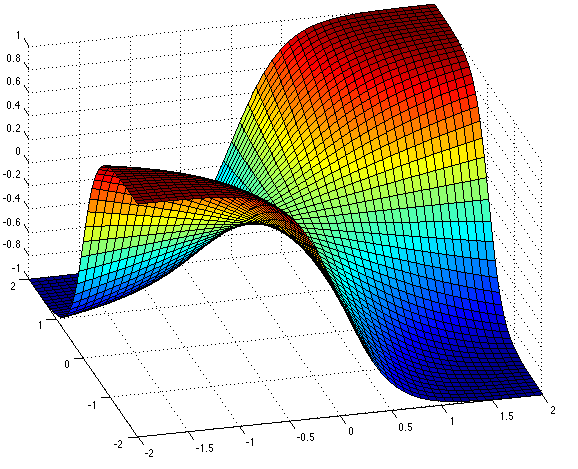
\includegraphics[width=0.5\textwidth]{sigmoid}
			\caption[Sigmoid Kernel]{
				\footnotesize{
					Sigmoid Kernel visualization in d = 3. \textit{Source:} \cite{carrington2014new}
				}
			}
			\label{fig:svm_sig_kernale}
		\end{figure}
		
		This kernel originates from Neural Networks, another Machine Learning algorithm. The kernel, when implemented, produces an SVM equivalent to a two-layer \hyperref[ann]{Perceptron Neural Network}. The calculation of the kernel function is shown in Equation \ref{equ:svm_sig_kernal}.
		\begin{equation}
			\mathlarger{K}(\textbf{x}_i,\textbf{x}_j) = \text{tanh}(\gamma \cdot \textbf{x}^T_i \textbf{x}_j + r)
			\label{equ:svm_sig_kernal}
		\end{equation}
		
	
	
	\paragraph{Margin Rigidity or Slack}
		Current research of SVMs revolves around the concept of \textit{Soft-Margins} (\cite{SVM_cortes1995support}). In the case of non-linearly-separable data, which is usually the case, a \textit{hinge loss} function is added to formula. Its purpose is to penalize for observations, which are on the 'wrong' side of the margin, that is between the support vectors. Using this method, observation are allowed to break the constraint present in the hard-margin case (Equation \ref{svm_opt_dist}). In other words, observations are permitted to cross to the "wrong side" of the margin, but they are being penalized for it, as demonstrated through the variable $c$ in Equation \ref{svm_soft_margin}. A trade-off between margin width, which represents the distinctness of each class, and the amount of misclassified observations can than be specified by the user.
	
		\begin{equation}
			\begin{aligned}
				max \ (c - y_i(\vec{w} \cdot \textbf{x}_i - b)), 
				\  \ \ \forall \ c = \ 
				\begin{cases} 
					0 \ \ \text{if} \ \ref{svm_constaints}\ \text{holds true}\\
					1 \ \ \text{else}
				\end{cases}
			\end{aligned}
			\label{svm_soft_margin}
		\end{equation}
	
		The optimization problem with the soft-margins approach is represented in Equation \ref{svm_sof_marg_opt}. The variable $\lambda$ controls the penalty magnitude for observations being on the wrong side of the margin. $\lambda$ therefore, represents the trade off between margin size and the observation being correctly classified. As the $\lambda$ approaches zero, the problem converges into the hard margin scenario.
	
		\begin{equation}
			\Bigg[
			\frac{1}{n} \sum_{i=1}^{n}max(c-y_i(\vec{w} \cdot \textbf{x}_i - b )) 
			\Bigg]
			+ \lambda || \vec{w} ||^2
			\label{svm_sof_marg_opt}
		\end{equation}
	
	\paragraph{Multiclass classification}
		The classification model in itself is natively used for binary stratification, that is 2 classes only. However, as may be the case in many classification scenarios, data often has more then 2 dimensions. For the purpose of Multiclass classification using SVMs, a process known as \textit{class-reduction} is implemented (\cite{aly2005survey}). This is done by either a 'one-vs-all' or 'one-vs-one' approach. With the former method, classifiers for each given class $c$ are trained to differentiate it from the rest of the set. The testing data is then inputed into each of the classifiers and the highest scoring one (having the largest distance from the decision boundary) determines the class for each observation. This is also known as the \textit{winner-takes-all} approach. Using the latter method consists of training classifiers for every combination of two classes out of all the classes. In the case where there are $n$ classes, $\frac{n(n-1)}{2} $ classifiers will be trained as in Equation \ref{one_v_one} with
		a max-wins voting strategy, whereby every observations is denoted to one of two classes by each classifier. Afterwards, the final classification is determined by a tally of the votes on each new data point.
		
		\begin{equation}
			\begin{aligned}
				\text{Classes:}	\ \ \ \ \ \ \ \	\textbf{c} &= (c_1,c_2,c_3,c_4) \\
				\text{Classifiers:}\ \ \ 	\textbf{Cl.} &= (Cl_{12},Cl_{13},Cl_{14},Cl_{23},Cl_{24},Cl_{34})
			\end{aligned}	
			\label{one_v_one}
		\end{equation}
	
	\paragraph{Strengths and Weaknesses}
		Among the advantages of SVMs one can mentions several factors. Firstly, the usage of different kernels - especially user-specified ones, allows for expert knowledge to be integrated into the classification problem. Secondly, the optimization space for the categorization problem is convex, thus making it easily and usually swiftly solvable with appropriate solving algorithms. And thirdly, the usage of soft-margins, or penalizing for error in classification makes the user more aware of the imminent over-fitting, which is the bane of classification problems. This awareness encourages the user to take a more cautious approach and avoid over-specification. The disadvantages include but are not limited to the following. The choice of kernel is for the user to decide, which could add to the element of human error, especially with dilettante users. Secondly, the problem of Multiclass classification is not solved directly, but rather is adopted for, by creating a multitude of partial SVMs (\ref{one_v_one}), making it not the most effective tool for such scenarios. Finally, the algorithm tends to be memory intensive during the training phase. Because a value needs to be calculated for each pair of $n$ points, a matrix of size $n^2$ must be constructed. For example, when training with a dataset of size $n = 1,000$ - the kernel values matrix will be $n^2 = 1,000,000$ large. In optimized modules though, you can get away with only calculating half of the matrix, since its symmetrical along its diagonal.

	\subsubsection{Artificial Neural Networks}
	An Artificial Neural Network (ANN) \cite{mcculloch1943logical} is a mathematical computational model, whose development was inspired by cognitional processes in a biological brain. This sort of network typically consists of numerous interconnected input and output information units. The form of connectivity between these units embodies the connection strength, in a fashion similar to how neurons are linked in the brain. ANNs are predominantly used in Cognitive Sciences and related software such as Artificial Intelligence Systems. Common tasks for such systems are character recognition, facial recognition, financial markets prediction and text mining among other uses.
	
	\paragraph{Intuition}
		A neural network is composed of linked processors called Perceprtons (combination of preception and neurons), each capable of executing a simple mathematical operation. However, when combined, said networks are capable of sophisticated problem solving. Any given Perceptron receives inputs $ i $ with according weights $ w $. The sum of all weighted inputs (products) is then calculated. When this sum exceeds a threshold value $ T $ the output $ O $ is equal to one and zero otherwise, as in [\ref{ann_neuron_sumprod}]. This operation resembles the operation of a biological neuron, which releases an electric signal when its agitation transcends a certain limit.
	
	\begin{equation}
		\langle i,w \rangle = \sum_j i_j w_j = 
			\begin{cases}
				1 \ \ \text{,  } \sum_j i_j w_j \geq T \\
				0 \ \ \text{,  } \sum_j i_j w_j < T 
			\end{cases}
		 = O
		\label{ann_neuron_sumprod}
	\end{equation}
	
	\begin{figure}[h]
		\centering
		\captionsetup{width=0.8\textwidth}
		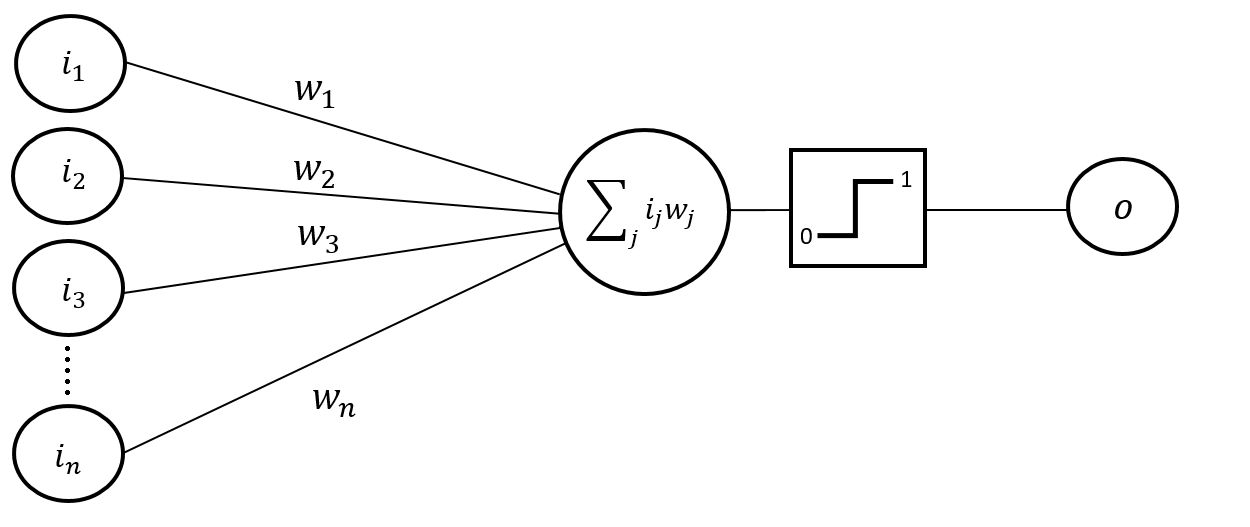
\includegraphics[width=0.8\textwidth]{ANN_percept.png}
		\caption[ANN Perceptron]{
			\footnotesize{
				Structure of a Perceptron with $ n $ input nodes $ i $ and output $ o $. Output 1 when threshold is surpassed and zero otherwise.
			}
		} 
		\label{ANN_percept}
	\end{figure}
	
	The organization of Perceptrons is crucial to the networks operation. The input weights are the ones, which determine the pattern to be recognized \cite{bishop1995neural}. Therefore, the prime objective when constructing an ANN is determining proper values for the weights. The Perceptrons are used as logical gateway, which can carry out the "AND" and "OR" operations. A major obstacle in the early days of ANNs was the inability to construct  a "XOR" (exclusive OR) logical gate, irregardless of the weights on the inputs. This difficulty was later overcome with the introduction of multi-layered ANN.
	
	Multi-layered ANNs consist of several layers of Perceptrons. All layers except the first (input layer) and the last (output layer) receive their inputs from the lower level of Perceptrons and output into the higher layer, which in turn uses this output as its input. It was demonstrated that a "XOR" gateway could be constructed using a 3-layered network [\ref{ANN_XOR}].
	
	\begin{figure}[h]
		\centering
		\captionsetup{width=0.8\textwidth}
		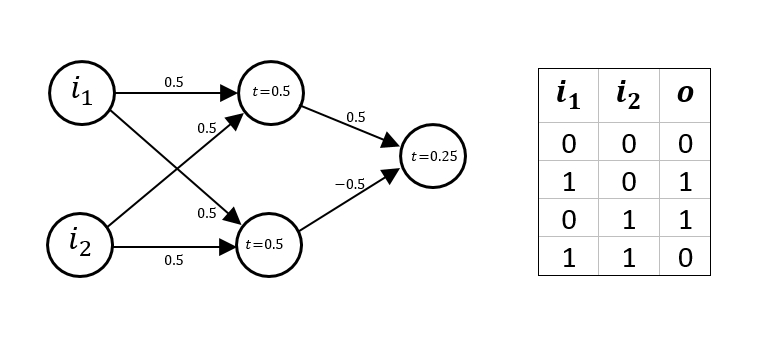
\includegraphics[width=0.8\textwidth]{ANN_XOR.png}
		\caption[ANN XOR Perceptron-Network]{
			\footnotesize{
				A three layer Network, creating a XOR gateway.
			}
		} 
		\label{ANN_XOR}
	\end{figure}	
	
	
	\paragraph{Classification}
		The type of network used most commonly for classification is a Multilayer Perceptron Network (MLP). This falls into the category of feedforward ANNs. A feedforward network, is such which does not allow cycles. Thus each layer only outputs information to the next layer, and not to the ones which came before. Typically a non-linear sigmoid function is used for activation rather than a binary step function as described in [\ref{ANN_percept}]. A sigmoid function [\ref{ann_sigmoid}] also often called a Soft Step or another continuous function are usually used, since ultimately the algorithm will have to calculate gradients to maximize or minimize an optimization function. Therefore this function should be continuous, differentiable and Real-valued.
		
		\begin{equation}
			\phi(x) = \frac{1}{1+ e^{-x}}
			\label{ann_sigmoid}
		\end{equation}
			
		\par
		
		The network is than optimized through the process of \textbf{Backpropogation} of errors. During the backwards propagation the initial weights of all the axons (input nodes of a neuron) weights are determined at random. Afterwards the optimization problem is set by measuring the aggregate error terms in classification (misclassification). This error is calculated as a function of all afore mentioned weights. This function thus needs to be minimized by observing the contribution of each weight to the error. In the next step, we take the gradient (derivative in vector space) and change the weights by $ \Delta w $ accordingly as shown in [\ref{ANN_backprop}]. We repeat this process until we no longer gets improvement (lower error terms) or the improvement is lower than a predetermined threshold.
		
		\begin{figure}[h]
			\centering
			\captionsetup{width=0.8\textwidth}
			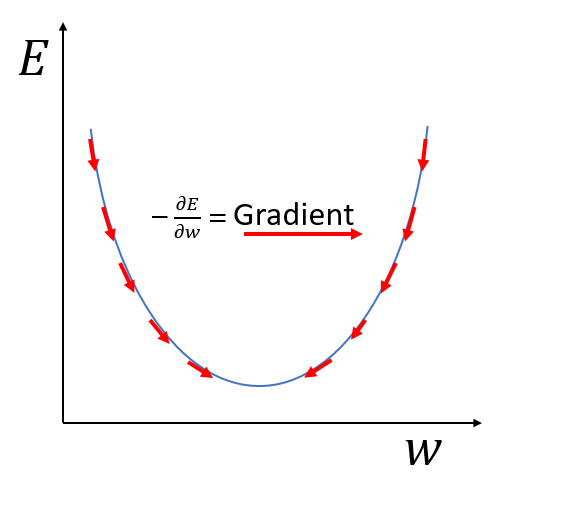
\includegraphics[width=0.5\textwidth]{grad_desc.png}
			\caption[ANN Gradient Descent]{
				\footnotesize{
					A descent down the error function, taking gradients of $ w $ to calculate the steps.
				}
			} 
			\label{ANN_backprop}
		\end{figure}
	
	\paragraph{Stochastic Gradient Descent}
		In the basic variant of ANN's  we optimize an objective function by tuning the weights in a manner which reduces the error term gradually with each iteration. With each repetition the weights are adjusted by $ \Delta w $ according to the gradient for each weight over all the observations. Every repetition  requires the calculation of the function's derivatives with respect to every data point and their summation within every iteration. This base method is also referred to as Batch Gradient Descent (BGD). This means, that in order to tune a weight $ w_j $ we must go through all its derivatives in the gradient and sum them up.  Applying this technique requires us to derive the function $ m \cdot n $ times in each iteration of the algorithm, with $ m $ being the number of data points and $ n $ the set of features. The problem with this procedure is its computational costliness which increases as the data set grows larger. Therefore the standard BGD approach scales poorly. We can hence modify the algorithm using a method called Stochastic Gradient Descent(SGD) to address scalability issues.
		
		\par
	
		To carry out SGD we first shuffle the training dataset in interest of safety since we want to try and avoid any inherit order present in the dataset. Subsequently, inside the spectrum of the first data point we derive each of the weight modification and adjust after each derivation. Than we continue and repeat this process for each data point. We are now adjusting after each derivation instead for all derivations of a data point. Therefore, the descent tempo is now $ (m \cdot n) \ \frac{\text{improvements}}{\text{algorithm round}}$ as compared to the tempo $(n) \ \frac{\text{improvements}}{\text{algorithm round}}$ of BGD. Finally, the loop over all the data points can be repeated more than once for better results.
		
		\par
		
		Since in each iteration we try and fit for a single data point of the dataset it is much more likely that the adjustment is not an improvement and actually takes us further (or not nearer) from the global minimum. Nonetheless, the algorithm does converge to the extremum and faster at that, then the BGD approach. I plot a graphical illustration of the algorithm convergence in [\ref{ann_sto_grad_desc}]. SGD is clearly recognizable with its "squiggly" line. One notable problem with this algorithm is that it might continuously overshoot the local minimum because of its high variance.
		
		\begin{figure}[H]
			\centering
			\captionsetup{width=0.8\textwidth}
			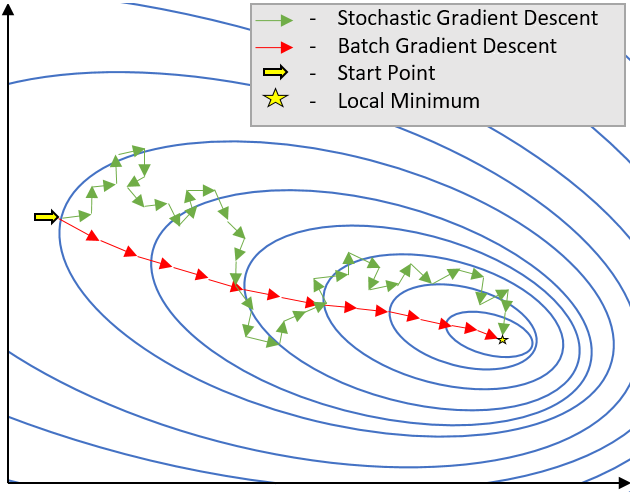
\includegraphics[width=0.5\textwidth]{sto_grad_desc.png}
			\caption[Batch and Stochastic Gradient Descent]{
				\footnotesize{
					A comparison of the Batch and Stochastic Gradient Descent Approaches 
				}
			} 
			\label{ann_sto_grad_desc}
		\end{figure}
	
		In the example above, a SGD approach is described, in which we fit the weights for a single observation at a time. It also possible to take very small batches of observations and fitting the algorithm on them. This approach is also known as Mini-Batch Gradient Descent and combines the best of both approaches, since it both addresses the overshooting complication of SGD and is much faster than BGD. Thus, by adjusting the batch size one can control the trade-off between speed and accuracy, where a larger batch should in a more accurate step, but the computation time will also increase. 
		
		\par
		
		The mechanism of Stochastic Gradient Descent at its core is extremely inaccurate on a single step basis, since the probability of improvement is much lower when compared to Batch Gradient Descent. This is compensated for with a much faster improvement rate, making the accumulated improvement catch up and overtake that of the normal scenario. The heightened convergence speed is what makes this approach more suitable for classification with extensive training data sets.
		
		\paragraph{Adaptive Moment Estimation}
			ADAM is another approach with can be used in tandem with SGD. Using ADAM we calculate the first (mean) and second (variance) moment of the gradients and modify the step size for each parameter (feature) in accordance with its frequency. Therefore, the update size is usually more significant for infrequent parameters and more fine for frequently occurring parameters.
			
		 

				
				
	\subsubsection{Decision Trees and Random Forests}
	Another popular type of classifiers stems from the idea of decision trees (\cite{quinlan2014c4}). That is, a flow chart consisting of decision intersections (called nodes) flows from a starting root (the tree stem). The data is further segmented in each following junction until a state is achieved, in which ideally all segments are "pure", containing observation belonging to a single class. Note that Decision Trees and other Ensemble Methods are not well suited for classification of \hyperref[data_sparsity]{sparse data}, due to the large number of features. This means the information gain from each note is very minor. A segment of a Decision Tree implemented in sparse data is graphically illustrated in Figure \ref{fig:rand_forest_sparse}.
	
	\begin{figure}[h]
		\centering
		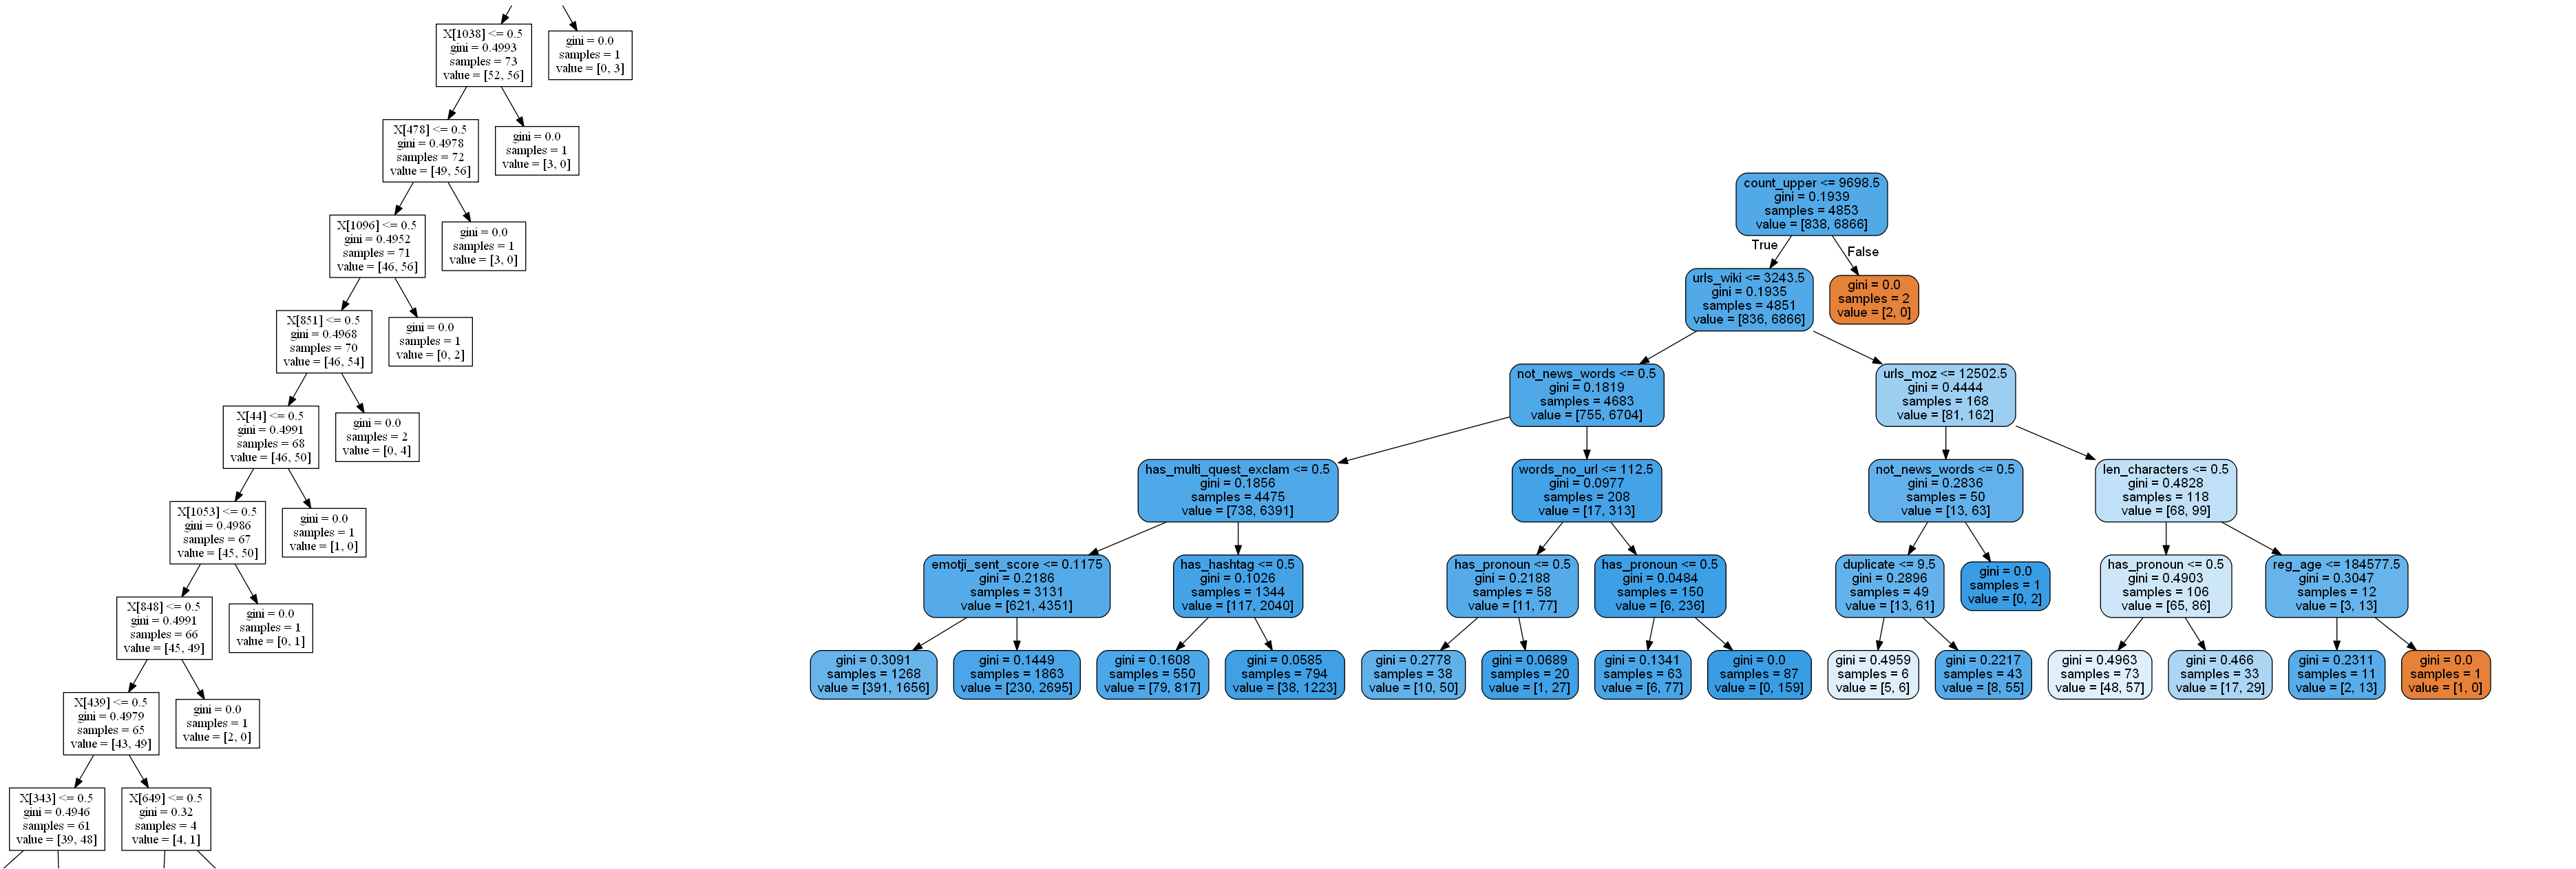
\includegraphics[width=1\textwidth]{decision_tree_sparse_data}
		\captionsetup{width=0.8\textwidth}
		\caption[Decision Tree with Sparse Data]{Decision Tree derived from sparse (Left) and non-sparse (Right) data}
		\label{fig:rand_forest_sparse}
	\end{figure}
		
	\paragraph{ID3 Algorithm} 
		This procedure of Decision Tree induction is known as the ID3 Algorithm (\cite{quinlan1986induction}). More formally, the design functions as follows. We start, as is common in classification problems, with a data training dataset. Each data point (observation) in the set has an assortment of attributes (features) and is assigned to a certain class. At each stage of the tree construction, including the inception stage, a node is created. This node receives as input a group of observations which belong to 2 or more classes. The node than selects a feature of the data and divides the data according to this feature. The feature selection consideration will be explained subsequently. For each possible value of the previously selected feature, a node is created. If the data inside a node belongs to a single class, it will not be segmented any further and the node will be denoted as a \textit{leaf}. If, on the other hand, the new node contains data points from different classes, we repeat the process of feature selection and segmentation accordingly. Finally, we want to reach a scenario in which, all leaves of the tree contain observations belonging to a single class each. The contents of such leaves may also referred to as \textit{pure subsets}.
		
	\paragraph{Entropy}
		The priorly mentioned decision rule for feature selection, upon which the data will be split in a given node, can be determined by 2 approaches. Both hold the same principle at their core, this being the amount of certainty gained from each split. Hence, the goal is the maximization of certainty, that after a given split, a data point belongs to one distinct class. For example, a feature would be considered a weak feature for splitting, if at a given node it splits the data in a manner where all subsets have relatively similar probabilities of belonging to the different classes. In such an example, no progress was made in the direction of segmenting the data completely. The closer the separation of the data brings us to pure subsets, the higher its ranking as a decision rule at a given node will be. This means, that the lower the entropy values are, the purer the resulting subsets will be.
		
		\par
		One measure which helps quantify the quality of this segmentation rule is \textbf{Entropy}. The calculation of Entropy is demonstrated in equation [\ref{dt_entropy}], with $ S $ being the subset passed to the node as input, $ i \in \{1:c \} $ denoting the different classes and $ p_i $ the percentage of data point corresponding to class $ i $. 
		
		\begin{equation}
			H(S) = \sum_{i=1}^c - p_i \cdot log_2 (p_i)
			\label{dt_entropy}
		\end{equation}
		
	 \paragraph{Gini}
	 	An alternative metric to entropy is the Gini Impurity coefficient. The coefficient denominates the probability of a randomly selected observation to be incorrectly labeled, if the label was set at random according to the actual distribution of labels in the dataset. We compute Gini by summing the probabilities of a given item belonging to a certain class $ i $ multiplied by the probability of misclassification. The Gini impurity is demonstrated in equation [\ref{dt_gini}], with $ i $ denoting a given class, out of $ c $ classes.
	 	
	 \begin{equation}
	 	\begin{aligned}
		 	I_G(p) &= \sum_{i=1}^c p_i(1-p_i) = \sum_{i=1}^c (p_i-p_i^2) \\  &=\sum_{i=1}^c p_i - \sum_{i=1}^c p_i^2 = 1 - \sum_{i=1}^c p_i^2 \\ &= \sum_{i \neq k} p_i p_k
	 	\end{aligned}
		\label{dt_gini}
	 \end{equation}
	 
	 \paragraph{Information Gain}	
	 	Entropy allows us to further calculate the "Information Gain" from each split. This gain is calculated in equation [\ref{dt_info_gain}], with $ S $ being the set of input examples, $ v $ a possible value of the attribute $ A $ and $ S_v $ the subset of $ S $ in which the $ A $ attribute of the examples is equal to $ v $. The gain is therefore, a weighted average of the Entropies, with respect to the prevalence of a given value $ v $ in each subset. Thus, Information Gain also assigns importance to the progress made from a new node. Ergo, a node which classifies few items purely might be outweighed by one which does not split into completely pure subsets, but rather splits correctly more items.
	 
			\begin{equation}
			Gain(S,A) = H(S) - \sum_{v \in values(A) } \frac{|S_v|}{S} H(S_v)
			\label{dt_info_gain}
	 \end{equation}
	 
	 \paragraph{Pruning}
		 After the tree is built, it undergoes the process of \textit{pruning}. This means, that branches which add little new information to the classification are removed. The algorithm is considered efficient and fast since, after pruning the amount of features actually used from a dataset is small. In addition, the algorithm is proficient in filtering noise and selecting the best features. Better data attributes are bound to have higher Information Gain values and are therefore more likely to be used in decision nodes.
	
	\paragraph{Random Forest}
		This algorithm builds a boot-strap system on the concept of Decision Trees. The algorithm by \cite{breiman1984classification} builds $ K $ different Decision Trees. Each Decision Tree $ T $ is built using a randomly picked subset $ S $ of the complete dataset. Each such tree is trained using the previously mentioned ID3 algorithm. However each tree does not use all the datasets attributes $ D $ but rather ones selected at random $ d << D $. The trees are not pruned. 
		
		\par
		As a consequence, each of the $ K $ trees is only suitable for a random subset $ S $ of the dataset and examines only a subset $ d $ of attributes. Each tree is not pruned, therefore it classifies its training data perfectly. When classifying novel data, the observation gets classified using all $ K $ tree, and the most commonly appearing classification decides the class. The process is therefore a voting classification using a \textit{Forest} of Decision Trees.
 
	
	


	
	
	
	
	
	
	
	
	
	
	
	
		
	